% -*- latex -*-
%%%%%%%%%%%%%%%%%%%%%%%%%%%%%%%%%%%%%%%%%%%%%%%%%%%%%%%%%%%%%%%%
%%%%%%%%%%%%%%%%%%%%%%%%%%%%%%%%%%%%%%%%%%%%%%%%%%%%%%%%%%%%%%%%
%%%%
%%%% This text file is part of the source of 
%%%% `Introduction to High-Performance Scientific Computing'
%%%% by Victor Eijkhout, copyright 2012-7
%%%%
%%%% This book is distributed under a Creative Commons Attribution 3.0
%%%% Unported (CC BY 3.0) license and made possible by funding from
%%%% The Saylor Foundation \url{http://www.saylor.org}.
%%%%
%%%%
%%%%%%%%%%%%%%%%%%%%%%%%%%%%%%%%%%%%%%%%%%%%%%%%%%%%%%%%%%%%%%%%
%%%%%%%%%%%%%%%%%%%%%%%%%%%%%%%%%%%%%%%%%%%%%%%%%%%%%%%%%%%%%%%%


\Level 0 {Perceptrons}

\Level 1 {Hyperplanes}

Given an input vector (feature vector)~$x$, we can compute a linear
function of the input
\[ y = w^tx. \]
(An affine function $y=w^tx+b$ can be accomodated by including a `bias
component' $x_n\equiv1$.)

This output $y$ can be used as a numerical value,
or as classification through
\[ 
\begin{cases}
  x\in C &\hbox{if $y\geq 0$}\\
  x\not\in C&\hbox{if $y<0$}\\
\end{cases}
\]

\Level 1 {Learning the coefficients}

Given an input and true output $(x^t,r^t)$ and a computed output
of~$y^t$, we have a squared error of
\[ E = \frac12 (r^t-y^t)^2 = \frac12 \left[r^t- w^tx^t\right]^2. \]
We train the weights
by finding a (local) minimum, characterized by
\[ 0=\frac{d E}{d x} = \bigl( \frac{\partial E}{\partial x_j} \bigr)_j
    = \bigl( (r-y)x_j \bigr)_j \]
This can be done with \indexterm{gradient descent}:
\[ w\leftarrow w+\Delta w \qquad
    \hbox{where $\Delta w=( \eta(r-y)x_j )_j$}. \]
where $\eta$ is a learning rate.


The linear function $y=w^tx$ is surprisingly useful. In fact, there is
a hard theoretical statement that says that enough of these functions,
followed by an appropriate normalization can approximate any
continuous function on a bounded domain.

\begin{quotation}
  \textsl{Universal Approximation Theorem}%
  \index{universal approximation theorem}

  Let $\varphi(\cdot)$ be a nonconstant,bounded, and
  monotonically-increasing continuous function. Let $I_m$ denote the
  $m$-dimensional unit hypercube $[0,1]^m$. The space
  of continuous functions on $I_m$ is denoted by
  $C(I_m)$. Then, given any function $f\in C(I_m)$
  and $\varepsilon>0$, there exists an integer
  $N$, real constants $v_i,b_i\in\mathbb{R}$ and
  real vectors $w_i \in \mathbb{R}^m$, where
  $i=1,\cdots,N$, such that we may define:
  \[
  F( x ) =
  \sum_{i=1}^{N} v_i \varphi \left( w_i^T x + b_i\right)
  \]
  as an approximate realization of the function $f$ where
  $f$ is independent of $\varphi$; that is,
  \[
  | F( x ) - f ( x ) | < \varepsilon
  \]
  for all $x\in I_m$. In other words, functions of the form
  $F(x)$ are dense in $C(I_m)$.
\end{quotation}

The function $y\leftarrow w^tx$ is called a \indextermdef{perceptron}.

\Level 1 {Linear discrimination}

A perceptron can be used to distinguish between two classes, by
looking at whether the output is positive or negative. This is
equivalent to using a `threshhold function' $s(\cdot)$ which takes
values 0,1 and looking at~$s(w^tx)$.

Often, the function~$s$ is taken as a sigmoid:
\[ \sigma(x) = \frac1{1+\exp{-w^tx}}. \]
(Note the appearance of such a function as~$\varphi$ in the approximation theorem
above.)

(Connection to posterior probability? Alpaydin~272)

\Level 0 {Multilayer networks}

Instead of a straightforward calculation $y\leftarrow w^tx$,
we can introduce a hidden layer as
\[ z_h = \sigma(w_h^tx) \]
and find the output~$y$ in terms of these hidden units:
\[ y_i = v_i^tz. \]

It is possible to introduce more than one hidden layer. This is often
a design decision, having a network that is `long and narrow' rather
than `short and fat'.

\Level 1 {Backpropagation}

\begin{figure}[ht]
  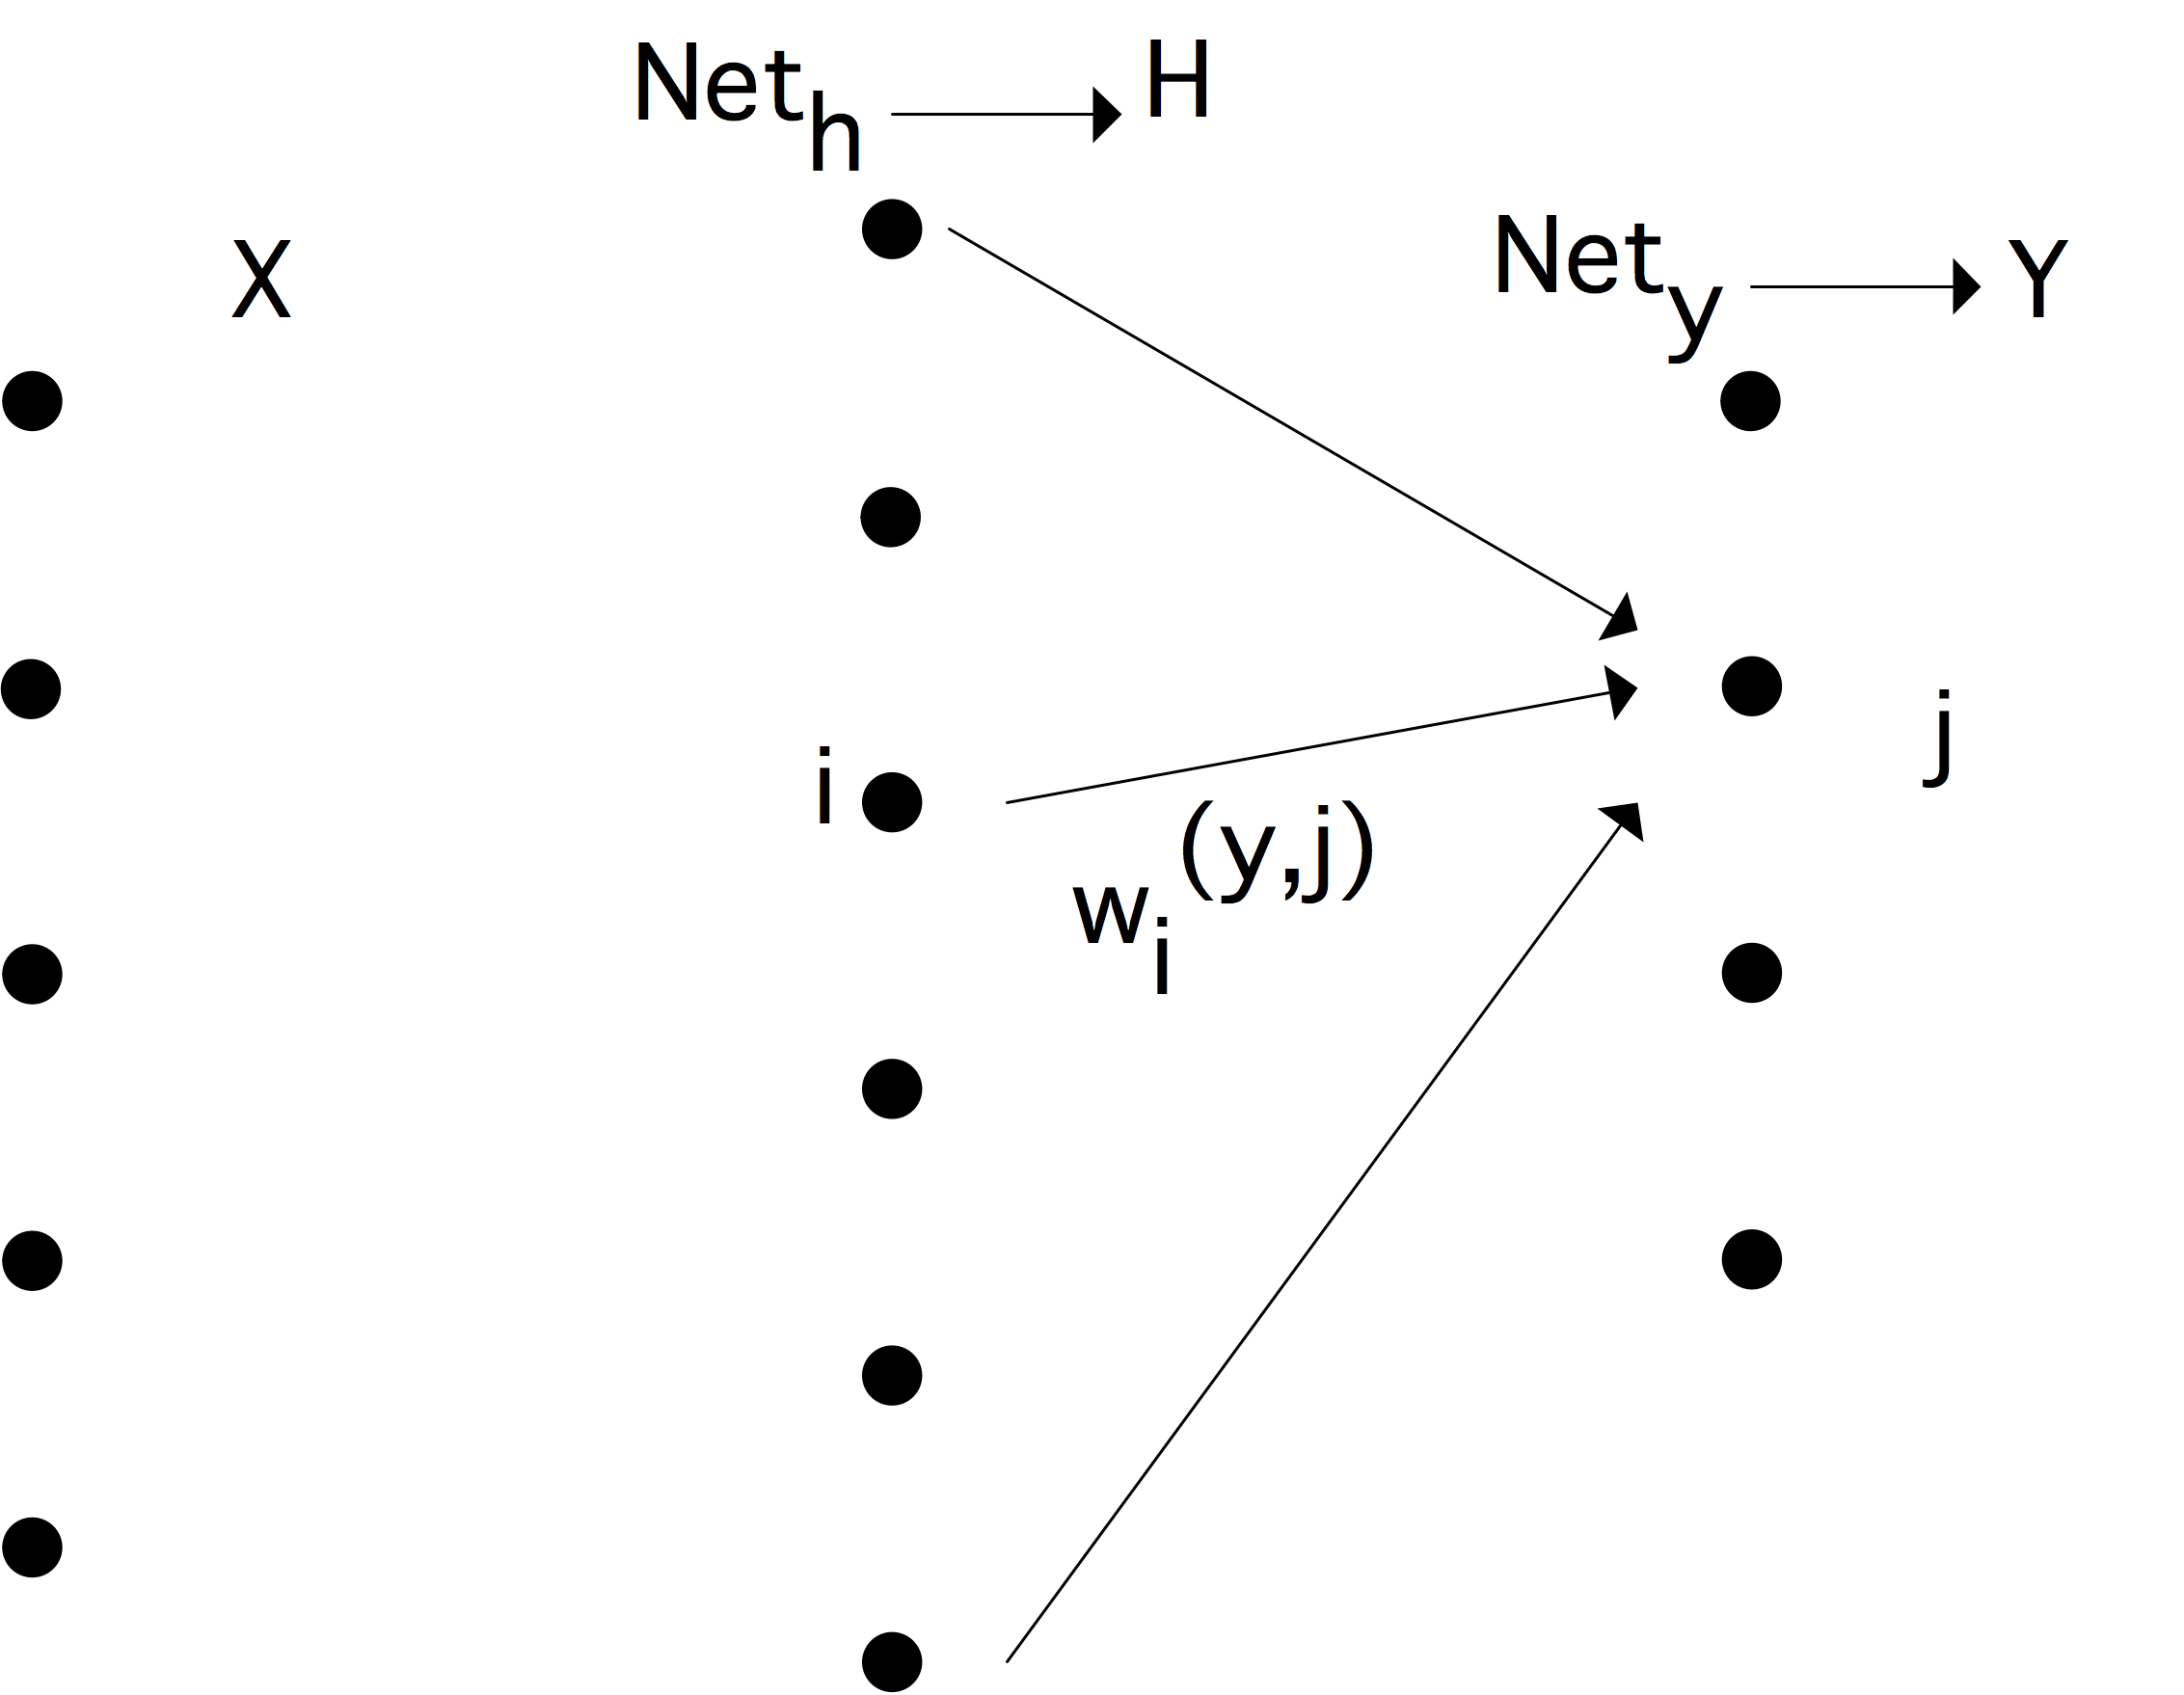
\includegraphics[scale=.12]{backpropagation-y}
  \caption{Back propagation, final layer coefficients}
  \label{fig:backprop-y}
\end{figure}

Let's describe a network with one hidden layer.
\def\net{\mathord{\mathit{Net}}}
\def\eE{{\cal E}}
\begin{itemize}
\item There is a set of inputs, $X$, of size~$n_x$.
\item On the intermediate layer,
  \[ \net^{(h)}= W^{ {(h)}^t }X \]
  where $W^{(h)}$ is a block of weight vectors:
  \[ \net^{(h)}_i = \sum_j w^{(h,i)}_jx_j. \]
\item The intermediate output values $H$ are formed with a sigmoid
  function:
  \[ h_i=\sigma\bigl(\net^{(h)}_i\bigr). \]
\item Net values on the output are computed from a second block of
  weights:
  \[ \net^{(y)}=W^{ {(y)}^t }H \]
  and we apply another sigmoid:
  \[ y_i=\sigma\bigl(\net^{(y)}_i\bigr). \]
\item We have a set of true output $T$ to compare against, and we
  measure the squared error
  \[ \eE=\frac12 E^tE,\qquad E=Y-T. \]
\end{itemize}

The problem is to compute the $W^{(h)}$ and $W^{(y)}$ coefficients to
minimize~$\eE$. We use some form of gradient descent.

The coefficients of the final layer are simple:
\begin{align}
  \frac{\partial\eE}{\partial w^{(y,j)}_i}
  &=E_j\frac{\partial y_j}{\partial w^{(y,j)}_i}
  &\hbox{$E_j$ is the only nonzero component}\\
  &=E_j \frac{\partial y_j}{\partial \net^{(y)}_j}
  \frac{\partial \net^{(y)}_j}{\partial w^{(y,j)}_i}
  &\hbox{chain rule}\\
  &=E_j y_j(1-y_j)
  \frac{\partial \net^{(y)}_j}{\partial w^{(y,j)}_i}
  &\hbox{use lemma~\ref{lemma:sigma-prime}}\\
  &=\delta_j h_i
  &\hbox{defining $\delta_j=E_jy_j(1-y_j)$}\\
\end{align}

In sum we get the update statement for the $j$-th colum of $W^{(y)}$
weights:
\[ W^{(y,j)} \leftarrow W^{(y,j)} - \epsilon \delta_j H \]
where $\epsilon$ is the learning rate.

For the intermediate layer coefficients we have to chain rule a couple
times more.

\begin{align}
  \frac{\partial\eE}{\partial w^{(h,j)_i}}
  &=\sum_{k=1}^{n_y} E_k\frac{\partial y_k}{\partial w^{(h,j)}_i}\\
  &=\sum_{k=1}^{n_y} \delta_k\frac{\partial \net^{(y)}_k}{\partial w^{(h,j)}_i}\\
  &=\sum_{k=1}^{n_y} \delta_k w^{(y,k)}_j
  \frac{\partial h_j}{\partial w^{(h,j)}_i}
  &\hbox{only $h_j$ contributes}\\
  &=\sum_{k=1}^{n_y} \delta_k w^{(y,k)}_j h_j(1-h_j)
  \frac{\partial \net^{(h)}_j}{\partial w^{(h,j)}_i}\\
  &=\sum_{k=1}^{n_y} \delta_k w^{(y,k)}_j h_j(1-h_j) x_i\\
\end{align}

We see that the final layer coefficients $W^{(y)}$ appear in this
formula for updating~$W^{(h)}$, which
is what gave this procedure the name \indextermdef{back propagation}.

\begin{figure}[ht]
  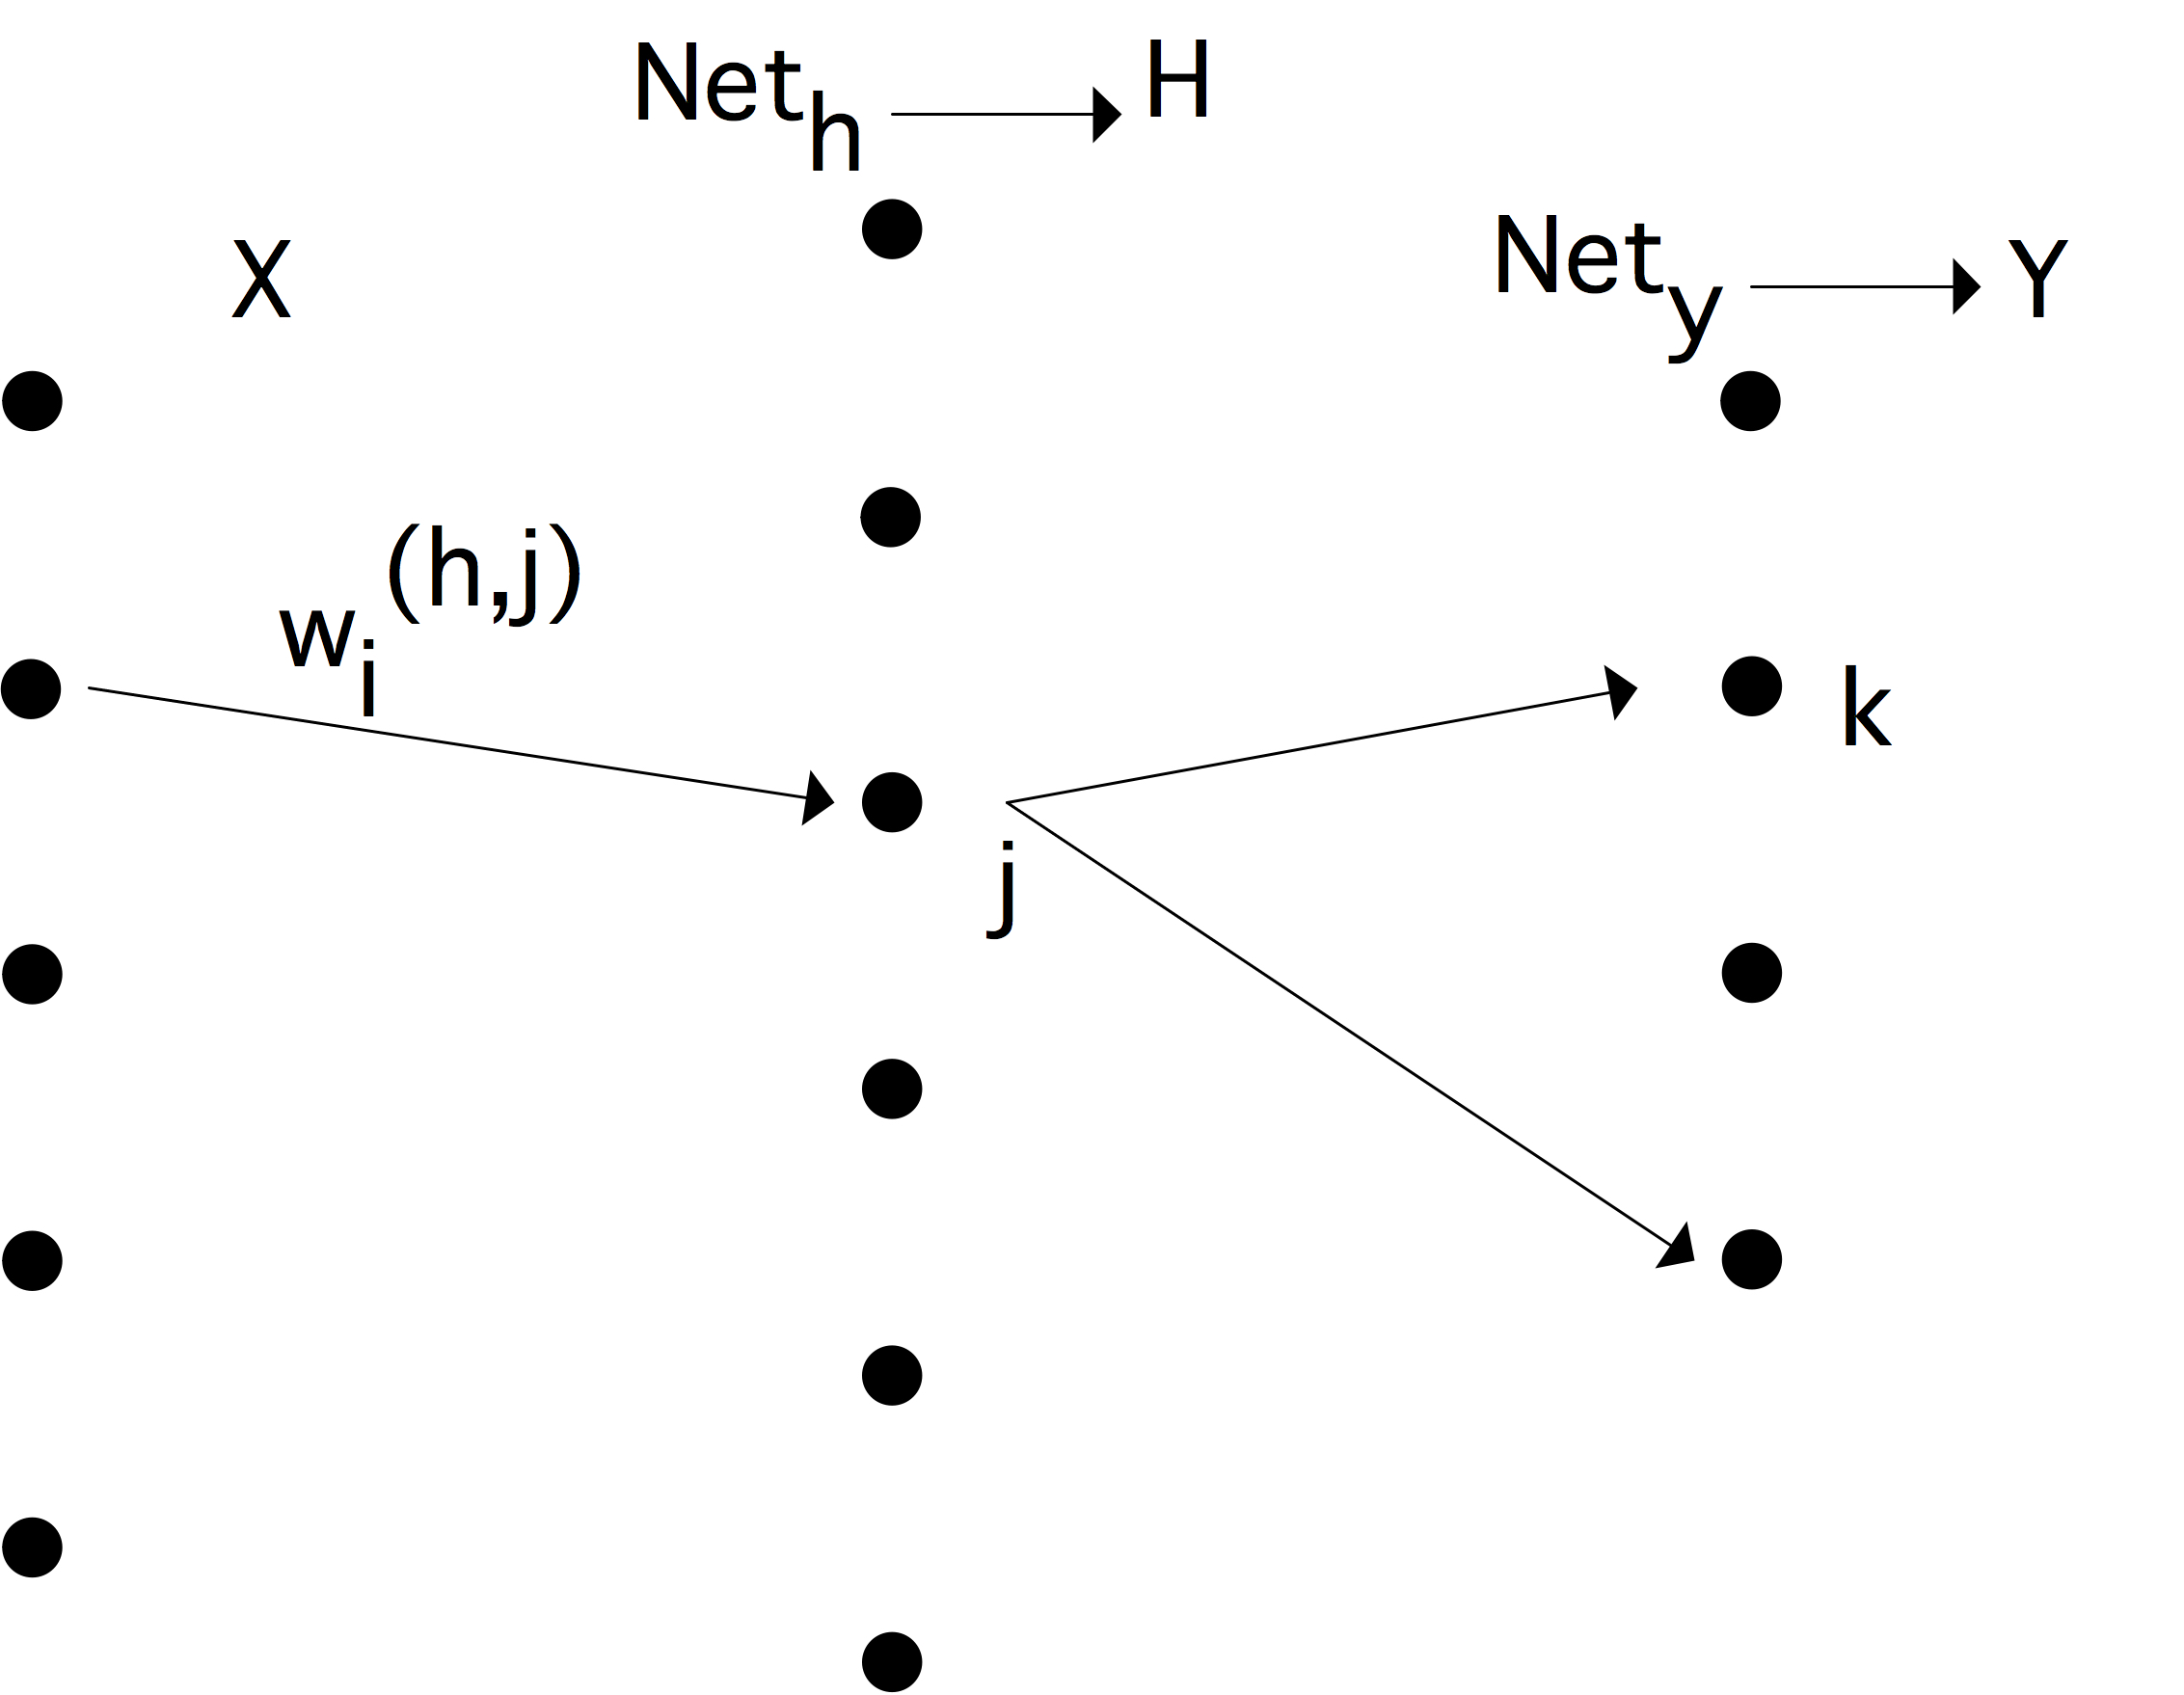
\includegraphics[scale=.12]{backpropagation-h}
  \caption{Back propagation, internal layer coefficients}
  \label{fig:backprop-h}
\end{figure}


\begin{lemma}
  \label{lemma:sigma-prime}
  \[ \sigma'(x) = \sigma(x)(1-\sigma(x)) \]
\end{lemma}
\begin{proof}
  \[
  \sigma'(x)=\frac{-1}{ (1+e^{-x})^2 }\cdot (-e^{-x})
  = \frac{e^{-x}}{ (1+e^{-x})^2 }
  = \frac{1}{ 1+e^{-x} } \frac{1+e^{-x}-1}{ 1+e^{-x} }
  \]
\end{proof}

For a worked out small example, see: \url{https://mattmazur.com/2015/03/17/a-step-by-step-backpropagation-example/}

\Level 0 {Computation}

GEMM in convolution kernels:
\url{https://petewarden.com/2015/04/20/why-gemm-is-at-the-heart-of-deep-learning/}
